%----------------------------------------------------------------------------------------
%	PACKAGES AND OTHER DOCUMENT CONFIGURATIONS
%----------------------------------------------------------------------------------------

\documentclass[11pt]{article}

\usepackage[utf8]{inputenc}
\usepackage[T1]{fontenc}
\usepackage[english, brazilian]{babel}

\usepackage{amsmath}
\usepackage{amsfonts}
\usepackage{amssymb}

\usepackage{appendix}
\usepackage[nottoc,numbib]{tocbibind}

\usepackage{graphicx}
\usepackage{kpfonts}
\usepackage{booktabs}
\usepackage{color}
\usepackage{listings}
\usepackage{icomma}

\usepackage{pdfpages}

% A bunch of defines:

\definecolor{Code}{rgb}{0,0,0}
\definecolor{Decorators}{rgb}{0.5,0.5,0.5}
\definecolor{Numbers}{rgb}{0.5,0,0}
\definecolor{MatchingBrackets}{rgb}{0.25,0.5,0.5}
\definecolor{Keywords}{rgb}{0,0,1}
\definecolor{self}{rgb}{0,0,0}
\definecolor{Strings}{rgb}{0,0.63,0}
\definecolor{Comments}{rgb}{0,0.63,1}
\definecolor{Backquotes}{rgb}{0,0,0}
\definecolor{Classname}{rgb}{0,0,0}
\definecolor{FunctionName}{rgb}{0,0,0}
\definecolor{Operators}{rgb}{0,0,0}
\definecolor{Background}{rgb}{0.98,0.98,0.98}

\lstset{
   frame = single, 
%  numbers = left,
   numberstyle = \tiny\color{blue},
   stepnumber = 3,
   breaklines = true,
%  language=Python,
   showstringspaces=false,
   formfeed=newpage,
%  tabsize=4,
%  commentstyle=\itshape,
   basicstyle=\ttfamily,
%  morekeywords={models, lambda, forms}
   numbers = left,
% Basic
   language = Python,
% Comments
   commentstyle=\color{Comments}\slshape,
% Strings
  stringstyle=\color{Strings},
  morecomment=[s][\color{Strings}]{"""}{"""},
  morecomment=[s][\color{Strings}]{'''}{'''},
% keywords
  morekeywords={import,from,class,def,for,while,if,is,in,elif,else,not,and,or,print,break,continue,return,True,False,None,access,as,,del,except,exec,finally,global,import,lambda,pass,print,raise,try,assert},
  keywordstyle={\color{Keywords}\bfseries},
}

\renewcommand{\appendixtocname}{Anexo}
\renewcommand{\appendixpagename}{Anexo}

\hyphenation{cross-over To-mas-si-ni al-go-rit-mos ma-ni-pu-la-ções ge-ra-rem}

\begin{document}

\begin{titlepage}

\newcommand{\HRule}{\rule{\linewidth}{0.5mm}} % Defines a new command for the horizontal lines, change thickness here

\center % Center everything on the page

%----------------------------------------------------------------------------------------
%	LOGO SECTION
%----------------------------------------------------------------------------------------


\includegraphics[scale=1.2]{ufulogo4}\\[1cm] % Include a department/university logo - this will require the graphicx package
 
%----------------------------------------------------------------------------------------

%----------------------------------------------------------------------------------------
%	HEADING SECTIONS
%----------------------------------------------------------------------------------------

%\textsc{\LARGE Universidade Federal de Uberlândia}\\[0.5cm] % Name of your university/college
\textsc{\Large Faculdade de Engenharia Elétrica}\\[0.6cm] % Major heading such as course name
{\large 8º trabalho de Inteligência Artificial}\\[0.5cm] % Minor heading such as course title

%----------------------------------------------------------------------------------------
%	TITLE SECTION
%----------------------------------------------------------------------------------------

\HRule \\[0.4cm]
{ \huge \bfseries Fundamentos de algoritmos genéticos}\\[0.4cm] % Title of your document
\HRule \\[1.5cm]
 
%----------------------------------------------------------------------------------------
%	AUTHOR SECTION
%----------------------------------------------------------------------------------------

\begin{minipage}{0.4\textwidth}
\begin{flushleft} \large
\emph{Aluno}\\
Roní G.\ \textsc{Gonçalves}\\% Your name
\end{flushleft}
\end{minipage}
~
\begin{minipage}{0.4\textwidth}
\begin{flushright} \large
\emph{Professor} \\
Keiji \textsc{Yamanaka}\\ % Supervisor's Name
\end{flushright}
\end{minipage}\\[0.1cm]
~
\begin{minipage}{0.85\textwidth}
\begin{flushleft} \large
10921EEL026 % Your name
\end{flushleft}
\end{minipage}\\[3cm]
~
% If you don't want a supervisor, uncomment the two lines below and remove the section above
%\Large \emph{Author:}\\
%John \textsc{Smith}\\[3cm] % Your name

%----------------------------------------------------------------------------------------
%	DATE SECTION
%----------------------------------------------------------------------------------------

{\large Uberlândia, \today}\\[1cm] % Date, change the \today to a set date if you want to be precise


\vfill % Fill the rest of the page with whitespace

\end{titlepage}

\setcounter{page}{2}

\newpage

\begin{abstract}
Um programa implementando os princípios básicos de algoritmos genéticos foi feito para se entender melhor como atuam os mecanismos de seleção, cruzamento e mutação numa população de números que são candidatos para minimizarem uma dada função $f(x)$.

\emph{Palavras-chave}: inteligência artificial, algoritmos genéticos, seleção, cruzamento, mutação.
\end{abstract}

\begin{otherlanguage}{english}
\begin{abstract}
An application that implements the fundamentals of genetic algorithms was developed in order to better understand the selection, crossover and mutation mechanisms in a population in which contains the candidates that minimize a given function $f(x)$.

\emph{Keywords}: artificial intelligence, genetic algorithms, selection, crossover, mutation.
\end{abstract}
\end{otherlanguage}

\newpage
\tableofcontents
\newpage

\section{Introdução}

Ao longo deste trabalho os mecanismos básicos presentes nos algoritmos genéticos são apresentados e exemplificados com código feito em Python.

Os mecanismos são unidos para resolverem um problema de minimização de uma função $f(x)$ proposto como exemplo no artigo de Marco Tomassini \cite{Tomassini}.

O primeiro processo é a criação de um primeiro conjunto de números binários gerados aleatoriamente; o segundo processo trata-se da seleção dos indivíduos mais aptos da geração anterior por meio da função de aptidão; em seguida, os indivíduos selecionados são aleatoriamente arranjados aos pares para que haja ou não o cruzamento entre eles de acordo com uma probabilidade de cruzamento $p_c$. Finalmente após todas essas etapas, de acordo com uma probabililidade $p_m$ de mutação os indivíduos originários do cruzamento de seus pais podem sofrer ou não mutação em algum de seus bits para que, a partir do processo de seleção, tudo se repita até que alguma condição seja alcançada. No presente trabalho, tal condição foi o número de gerações criadas.

Como exemplo de aplicação, tal algoritmo foi usado para encontrar o valor mínimo ou, pelo menos, um valor próximo ao mínimo da função $f(x) = - \left| x \sin{\sqrt{\left| x\right| }}\right| $ dentro do intervalo\footnote{Tal intervalo é escolhido somente para números pares devido à natureza simétrica da função $f(x)$.} de 0 a 512, isto é, encontrar $x^*$:

\begin{equation*}
f(x^*) = \min \{ f(x) ~ | ~ \forall x \in [0; 512] \}
\end{equation*}

Tomando $g(x) = - f(x)$, podemos transformar o problema anterior num de maximização de $g(x)$. Isso é feito para simplificar o algoritmo de forma a termos sempre valores positivos para as probabilidades calculadas futuramente. No entanto, o valor de $x^*$ que maximiza $g(x)$ é o mesmo que minimiza $f(x)$, pois os problemas são equivalentes:

\begin{equation*}
g(x^*) = \max \{ g(x) ~ | ~ \forall x \in [0; 512]\}
\end{equation*}

O gráfico das funções $f(x)$ e $g(x)$ podem ser visualizados nas figuras \ref{fig:fdexis} e \ref{fig:gdexis}.

\begin{figure}
\centering
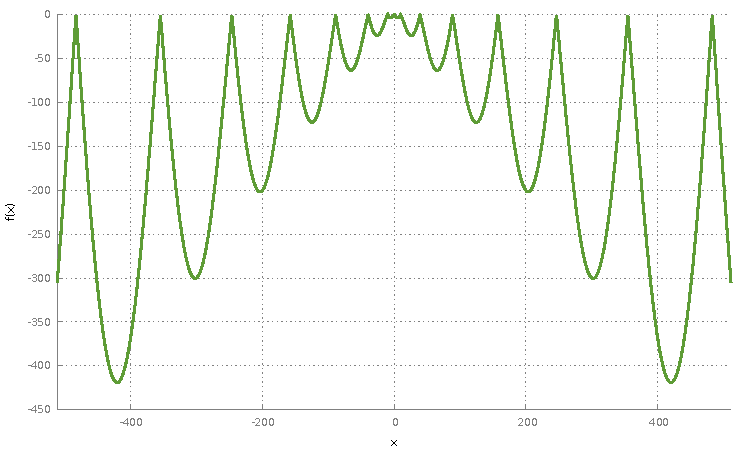
\includegraphics[scale=1]{../gnuplot/fdexis}
\caption{Gráfico da função $f(x)$ no intervalo de -512 a 512.}\label{fig:fdexis}
\end{figure}

\begin{figure}
\centering
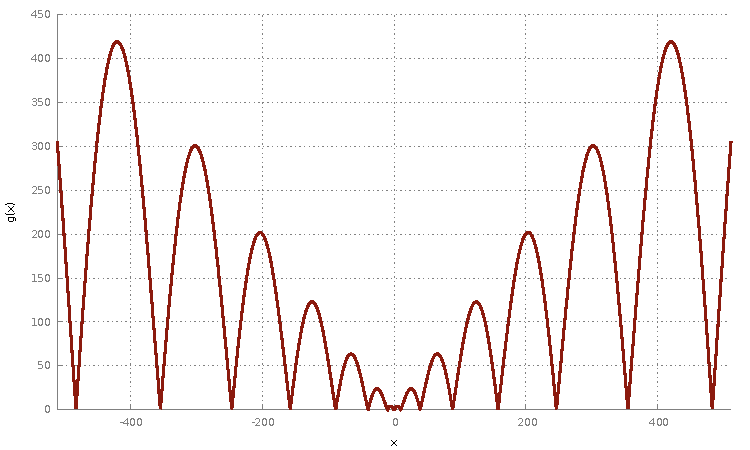
\includegraphics[scale=1]{../gnuplot/gdexis}
\caption{Gráfico da função $g(x)$ no intervalo de -512 a 512.}\label{fig:gdexis}
\end{figure}

Pela análise do gráfico, percebe-se que o máximo ou o mínimo das funções é próximo de 400. Na verdade, o valor real é 421.

\section{Gerando aleatoriamente a primeira geração $G_0$}

Duas funções são usadas para criar a primeira geração constituída de \emph{strings} contendo zeros e uns representando, em binário, os números candidatos a serem o valor que maximiza $g(x)$.

A primeira função, \texttt{gera\_individuo\_aleatorio()}, apenas seleciona nove\footnote{Para que haja 512 combinações diferentes de zeros e uns, são necessários nove dígitos binários: $2^9 = 512$. Porém, dessa forma o número 512 não fica representado, pois com nove dígitos binários podemos representar 512 números de 0 a $511 = 2^9 - 1$.} vezes de forma pseudo-aleatória um dos caracteres -- 0 ou 1 -- da \emph{string\_base}.

Enquanto que a segunda função, \texttt{gera\_populacao()}, usa a primeira função para preencher uma lista com um número de indivíduos igual ao parâmetro \emph{TamanhoDaPopulacao}.

\begin{lstlisting}
def gera_individuo_aleatorio():
	
	return (''.join(random.choice(string_base) for j in range(TamanhoDaString)))

def gera_populacao(TamanhoDaPopulacao):
	
	a = []
	
	for i in range(TamanhoDaPopulacao):
		a.insert(i, gera_individuo_aleatorio())
	
	return a
\end{lstlisting}

\section{Calculando a função de aptidão e probabilidades de cada indivíduo da população}

Antes de se aplicar a função de aptidão, é necessário fazer algumas manipulações com os indivíduos, pois eles são representados por \emph{strings} contendo apenas zeros e uns tais como: "000101010", "000011001",  "000001101"\ldots

Essas \emph{strings} são convertidas em números decimais pela seguinte função:

\begin{lstlisting}
def binario_em_decimal(Lista):
	
	a = []
	
	for i in range(len(Lista)):
		a.insert(i, int(Lista[i], 2))
	
	return a
\end{lstlisting}

Após passar por esta função, os indivíduos são representados por números decimais\footnote{Evidentemente que dentro do computador todos os números são representados de forma binária e não decimal.} tais como: 42, 25, 13\ldots \ e agora podem ser enviados à função que calcula suas aptidões.

\subsection{Função de aptidão}

Também conhecida em inglês por \emph{fitness}, a função de aptidão é aquela que avalia o valor de $x_i$, candidato a máximo de $g(x)$, e nos dá a medida de quão bom o i-ésimo candidato é. Nesse caso, a função de aptidão é a própria função $g$ e quanto maior o valor de $g(x_i)$, melhor é o candidato $i$. Temos, então, que:

\begin{equation*}
f_{aptidao} = \left| x \sin{\sqrt{\left| x\right| }}\right|
\end{equation*}

O que, em Python, pode ser escrito como:

\begin{lstlisting}
def calcula_aptidao(Cromossomo_Individuo):

	return (abs((Cromossomo_Individuo)*(sin(sqrt(Cromossomo_Individuo)))))
\end{lstlisting}

Vale lembrar que o valor de \texttt{Cromossomo\_Individuo} é aquele calculado pela função \texttt{binario\_em\_decimal()}.

\subsubsection{Dicionários ou \emph{hashes}}

Uma geração qualquer $G_i$ é representada, em Python, por uma lista contendo seus indivíduos. A lista tem o tamanho igual ao número de indivíduos contidos na geração $G_i$. Cada um deles pode ser acessado por meio de seus respectivos índices que vão de 0 até (Número de indivíduos $- 1$). Por exemplo: numa lista chamada \texttt{pop}, o primeiro elemento dela é acessado como \texttt{pop[0]}.

No entanto, essa maneira de guardar a identidade do indivíduo e o seu valor é insuficiente para atrelá-lo ao valor de sua função de aptidão. Para fazer isso, usou-se uma estrutura de dados nativa do Python chamada dicionário ou, em inglês, \emph{hash}.

Os dicionários são um conjunto de pares do tipo (chave, valor). Para este problema específico as chaves são os índices que representam cada indivíduo de uma certa geração da lista; os valores são os resultados da função de aptidão bem como as probabilidades calculadas subseqüentemente como se verá a seguir.

Por meio, então, dos dicionários é possível associar a um indivíduo qualquer a sua função de aptidão:

\begin{lstlisting}
def associa_aptidao(Populacao):	

	dicionario = {}

	for i in range(len(Populacao)):
		
		dicionario[i] = calcula_aptidao(Populacao[i])	

	return dicionario
\end{lstlisting}

\subsection{Probabilidades dos indivíduos serem selecionados}

A função de aptidão já mede o quão bons são os candidatos a máximo. É necessário ainda que, para cada candidato, seja atribuída uma probabilidade de ser selecionado proporcional ao valor de sua função de aptidão. Isso é feito em três passos:

\begin{enumerate}
\item Para cada geração, calcula-se a soma $S$ dos valores da função de aptidão de todos os seus indivíduos;
\item Para cada indivíduo, calcula-se a probabilidade $p_i$ como sendo a razão entre sua função de aptidão e S e a associa ao respectivo indivíduo;
\item Cria-se uma "roleta" \ contendo $c_i$, as somas parciais e sucessivas de $p_i$.
\end{enumerate}

As equações referentes ao passo-a-passo anterior são:

\begin{equation*}
S = \sum_{i = 1}^{TamGeracao} g(x_i)
\end{equation*}

\begin{equation*}
p_i = \frac{g(x_i)}{S}
\end{equation*}

\begin{equation*}
c_i = \sum_{k = 1}^{i} p_k, ~~~ i = 1, 2, 3,\ldots, TamanhoDaGeracao 
\end{equation*}

O código da função que realiza o primeiro passo é como se segue:

\begin{lstlisting}
def calcula_aptidao_total(Dicionario):

	aptidao_total = 0
	
	for i in range(len(Dicionario)):
	
		aptidao_total = aptidao_total + Dicionario[i]
	
	return aptidao_total
\end{lstlisting}

A função que executa o segundo passo pode ser escrita como:

\begin{lstlisting}
def associa_probabilidade(Dicionario, AptidaoTotal):

	for i in range(len(Dicionario)):
		
		Dicionario[i] = Dicionario[i]/AptidaoTotal
	
	return Dicionario
\end{lstlisting}

O último passo é conseguido como mostra a próxima função \texttt{associa\_prob\_cumulativa()}:

\begin{lstlisting}
def associa_prob_cumulativa(Dicionario):

	prob_acumulada = 0
	
	for i in range(len(Dicionario)):
		
		prob_acumulada = prob_acumulada + Dicionario[i]
		
		Dicionario[i] = prob_acumulada
	
	return Dicionario
\end{lstlisting}

\section{Selecionando os indivíduos da próxima geração}

Tendo todas as probabilidades dos indivíduos calculadas e associadas a eles, resta apenas selecionar quais serão os escolhidos para cruzarem e gerarem os novos indivíduos da próxima geração.

\begin{lstlisting}
def seleciona(Populacao, Dicionario):
	
	PopulacaoSelecionada = []
	
	DicionarioAuxiliar = {}
	
	ListaAuxiliar = []
	
	ListaAuxiliar = Dicionario.values()
	
	indice = 0
	
	for i in range(len(Dicionario)):
		
		DicionarioAuxiliar[Dicionario[i]] = i	
	
	for i in range(len(Populacao)):
		
		numero_aleatorio = random.uniform(0.0,1.0)
		
		ListaAuxiliar.append(numero_aleatorio)
		
		ListaAuxiliar.sort()
		
		indice = ListaAuxiliar.index(numero_aleatorio)
		
		if(indice == (len(ListaAuxiliar) - 1)):
		
			indice = indice - 1
		
		ListaAuxiliar.remove(numero_aleatorio)
		
		PopulacaoSelecionada.insert(i, Populacao[DicionarioAuxiliar[ListaAuxiliar[indice]]])
	
	return PopulacaoSelecionada
\end{lstlisting}

\subsection{Princípio de funcionamento da roleta}

Ao obter as probabilidades acumuladas $c_1$, $c_2$, $c_3$, forma-se um tipo de gráfico de setores. Usando-se a função \texttt{random.uniform()}, obtém-se um número $r$ aleatório que é comparado aos $c_i$ de tal forma que se $c_0 < r \leqslant c_1$, então o indivíduo selecionado será aquele correspondente ao índice 1.

\section{Cruzando os indivíduos selecionados}

Uma vez que os indivíduos de uma dada geração $n$ são selecionados, eles são arranjados aleatoriamente aos pares e cruzados para formarem os indivíduos da próxima geração $n+1$. É importante notar que, nesse processo de seleção e cruzamento, os pais originais são perdidos para sempre.

O cruzamento, ou melhor, a troca de informações entre os pais se dá da seguinte forma: um número aleatório entre zero e o valor do índice do penúltimo elemento da \emph{string} que representa um indivíduo é escolhido e a partir desse índice duas \emph{substrings} são criadas contendo uma parte da informação original dos "pais"; após isso, elas são comutadas entre os pais criando os filhos.

Algumas conversões de tipos acontecem por conta da escolha da estrutura de dados feita para representar a informação genética que cada indivíduo carrega. Em Python, os elementos de uma \emph{string} podem ser acessados individualmente, porém eles não podem ser alterados. Assim, as \emph{strings} são convertidas em listas que permitem não só acessar seus membros pelos índices, como também alterá-los. Feitas todas as alterações na informação dos indivíduos eles são novamente convertidos em \emph{strings} por meio do método \texttt{join()}.

Além disso, o cruzamento não ocorre sempre. Na verdade, ele pode ocorrer se um número aleatório dentro de uma distribuição uniforme com valores entre 0 e 1 for maior que o valor definido para a probabilidade de cruzamento $p_c$ que, nesse caso, vale $0,6$.

\begin{lstlisting}
def cruza(Populacao):

	pai = ""
	mae = ""
	
	indice_pai = random.choice(range(len(Populacao)))

	indice_mae = random.choice(range(len(Populacao)))
	
	pai = Populacao[indice_pai]
	mae = Populacao[indice_mae]
	
	indice_cruzamento = random.choice(range(0,(len(pai)-2)))
	
	pai = list(pai)
	mae = list(mae)
	
	for i in range(indice_cruzamento, len(pai)):
		
		aux = ''
		
		aux = pai[i]
		
		pai[i] = mae[i]
		
		mae[i] = aux
	
	pai = ''.join(pai)
	mae = ''.join(mae)
	
	Populacao[indice_pai] = pai
	Populacao[indice_mae] = mae
	
	return Populacao
\end{lstlisting}

\section{Mutando os indivíduos de uma geração}

A mutação é o último mecanismo que age sobre uma nova geração, logo após ela ser formada por meio do cruzamento dos indivíduos selecionados da geração anterior. Ela pode ou não acontecer; para cada indivíduo e para cada bit\footnote{Nesse caso, na verdade, é para cada caractere que compõe a \emph{string}.} que compõe o cromossomo do elemento da população, é sorteado um número aleatório entre zero e um de uma distribuição uniforme -- usa-se a função \texttt{random.uniform(0.0,1.0)} -- e caso o número aleatório sorteado seja maior que a probabilidade $p_m$ de mutação, então o indivíduo terá seus genes mutados. A probabilidade de mutação vale $0,01$.

\begin{lstlisting}
def muta(Populacao):
	
	indice_populacao = random.randint(0, (len(Populacao)-1))
	
	auxilio = Populacao[indice_populacao]
	
	auxilio = list(auxilio)
	
	indice_individuo = random.randint(0, (len(auxilio)-1))
	
	if (auxilio[indice_individuo] == '1'):
		
		auxilio[indice_individuo] = '0'
	
	else:
		auxilio[indice_individuo] = '1'
	
	auxilio = ''.join(auxilio)

	Populacao[indice_populacao] = auxilio
	
	return Populacao
\end{lstlisting}

\section{Resultados}\label{sec:resultados}

Nesta seção, são apresentados alguns dos resultados obtidos variando-se alguns dos inúmeros parâmetros possíveis deste algoritmo. Um fato importante de ser notado é a natureza parcialmente aleatória dos resultados obtidos. Isso significa que após a execução do programa, não necessariamente o valor $x^*$ que minimiza a função $f(x)$ será realmente encontrado: pode-se encontrar um valor razoavelmente próximo.

Um esquema simplificado do algortimo usado é mostrado nos passos abaixo:

\begin{enumerate}
\item Cria $n$ indivíduos aleatórios para compor a geração inicial $G_0$;

\item Enquanto o número de gerações for menor que um valor mínimo estipulado, faça:

\begin{enumerate}
\item Calcula a função de aptidão de cada indivíduo;

\item Calcula a probabilidade de cada indivíduo;

\item De acordo com a probabilidade calculada, seleciona indivíduos para comporem a próxima geração;

\item Aleatoriamente cruza os indivíduos selecionados;

\item A partir do resultado dos cruzamentos, cria a nova geração;

\item Aplica a mutação sobre a nova geração.
\end{enumerate}
\end{enumerate}

\subsection{Variação do número de gerações}

Ao variar a quantidade de gerações dois aspectos aparecem: (1) o aumento do número de gerações não garante que o mínimo ou máximo da função seja encontrado. Isto significa, por exemplo, que o valor mínimo da função $f(x)$, 421, pode ser encontrado na execução do algoritmo com $n = 50$ no passo 1 e, às vezes, esse mesmo mínimo não será encontrado caso o programa execute novamente com $n = 1000$; (2) apesar de a presença do melhor indivíduo não ser garantida pelo aumento do número de gerações criadas, tal aumento tende a melhora a aptidão média da população.

\subsection{Variação do número de indivíduos de uma população}

Nas tabelas que se seguem, os indivíduos da última geração $G_{69}$ são mostrados. Os parâmetros probabilidade de cruzamento $p_c$, probabilidade de mutação $p_m$ e quantidade de gerações criadas foram mantidos constantes e iguais a $0,6$, $0,01$ e $70$ respectivamente. Nesses testes, o único parâmetro a ser alterado foi o número de indivíduos (5, 10, 15 e 20) para cada tabela.

\begin{table}[h]
\centering
\begin{tabular}{cc}
 teste & indivíduos \\ 
 \midrule 
 1 & $[367, 367, 367, 367, 367]$ \\ 
 2 & $[198, 198, 198, 198, 198]$ \\ 
 3 & $[291, 291, 291, 291, 291]$ \\ 
 4 & $[280, 280, 280, 280, 280]$ \\ 
 5 & $[407, 407, 407, 407, 407]$ \\
 \bottomrule
\end{tabular}\caption{5 execuções do mesmo programa com uma população composta por 5 membros.}
\end{table}

\begin{table}[h]
\centering
\begin{tabular}{cc}
 teste & indivíduos \\ 
 \midrule 
 1 & $[294, 294, 294, 294, 294, 294, 294, 294, 294, 294]$ \\ 
 2 & $[320, 320, 320, 320, 320, 320, 320, 320, 320, 320]$ \\ 
 3 & $[407, 407, 407, 407, 407, 407, 407, 407, 407, 407]$ \\ 
 4 & $[421, 421, 421, 421, 421, 421, 421, 421, 421, 421]$ \\ 
 5 & $[459, 459, 459, 459, 459, 459, 459, 459, 459, 459]$ \\
 \bottomrule
\end{tabular}\caption{5 execuções do mesmo programa com uma população composta por 10 membros.}
\end{table}

\begin{table}[h]
\centering
\begin{tabular}{cc}
 teste & indivíduos \\ 
 \midrule 
 1 & $[426, 426, 426, 426, 426, 426, 426, 426, 426, 426, 426, 426, 426, 426, 426]$ \\ 
 2 & $[426, 426, 426, 426, 426, 426, 426, 426, 426, 426, 426, 426, 426, 426, 426]$ \\ 
 3 & $[432, 432, 432, 432, 432, 432, 432, 432, 432, 432, 432, 432, 432, 432, 432]$ \\ 
 4 & $[441, 441, 441, 441, 441, 441, 441, 441, 441, 441, 441, 441, 441, 441, 441]$ \\ 
 5 & $[430, 430, 430, 430, 430, 430, 430, 430, 430, 430, 430, 430, 430, 430, 430]$ \\
 \bottomrule
\end{tabular}\caption{5 execuções do mesmo programa com uma população composta por 15 membros.}
\end{table}

\begin{table}[h]
\centering
\begin{tabular}{cc}
 teste & indivíduos \\ 
 \midrule 
 1 & $[418, 423, 423, 418, 418, 418, 423, 423, 423, 418, $\\
   & $418, 418, 418, 418, 418, 418, 418, 418, 418, 418]$ \\
   & \\
 2 & $[410, 414, 410, 410, 410, 410, 410, 410, 410, 410, $\\
   & $410, 410, 410, 410, 410, 410, 410, 410, 410, 410]$ \\
   & \\
 3 & $[427, 427, 427, 427, 427, 427, 427, 427, 427, 427, $ \\
   & $427, 427, 427, 427, 427, 427, 427, 427, 427, 427]$ \\
   & \\
 4 & $[432, 434, 434, 432, 432, 432, 434, 432, 432, 432, $ \\
   & $434, 434, 434, 432, 432, 434, 434, 434, 434, 432]$ \\
   & \\
 5 & $[424, 424, 424, 424, 424, 424, 424, 424, 424, 424, $ \\
   & $424, 424, 424, 424, 424, 424, 424, 424, 424, 424]$ \\
 \bottomrule
\end{tabular}\caption{5 execuções do mesmo programa com uma população composta por 20 membros.}
\end{table}

\subsection{Variação das probabilidades de cruzamento e de mutação}

\subsubsection{Probabilidade total de cruzamento}

No caso em que todos os indivíduos selecionados de uma geração $n$ se cruzem para originar a geração $n+1$, não há um comprometimento tão grande dos resultados obtidos. Isso mostra que, para este problema, uma condição "generosa" de ocorrência de cruzamentos não é algo tão crítico assim. Como exemplo, mostra-se a geração final após a execução do programa com $p_m = 0,01$ e número de geração limite igual a 70: 422, 422, 422, 422, 418, 422, 420, 421, 422, 422, 418, 422, 422, 418, 422, 422, 422, 430, 430, 418, 422, 418, 421, 422, 422, 438, 418, 422, 422, 422, 418, 420, 422, 418, 418, 434, 438, 420, 426, 422, 422, 422, 428, 438, 418, 422, 422, 421, 422, 422, 422, 422, 422, 422, 422, 422, 430, 422, 422, 422, 418, 422, 426, 422, 422, 430, 418, 420, 422, 428, 418, 418, 422, 422, 418, 422, 430, 422, 422, 422, 434, 422, 422, 422, 418, 418, 418, 422, 422, 422, 422, 430, 422, 422, 422, 422, 422, 422, 418, 422.

\subsubsection{Diminuição da probabilidade de cruzamento}

\subsubsection{Probabilidade total de mutação}

Com uma probabilidade de 100\% de ocorrer mutação, o "ambiente" em que os indivíduos vivem é muito extremo e faz com que um resultado razoável não seja alcançado. Numa execução com $p_c = 0,6$ e o limite de gerações igual a 70, a última geração obtida com 100 indivíduos foi: 209, 195, 195, 211, 214, 195, 195, 195, 193, 195, 195, 211, 211, 211, 211, 198, 214, 195, 193, 193, 211, 197, 211, 195, 198, 198, 195, 195, 211, 195, 195, 211, 195, 209, 195, 198, 195, 198, 195, 195, 195, 197, 214, 195, 195, 193, 209, 195, 197, 193, 195, 195, 198, 211, 211, 195, 195, 195, 195, 195, 211, 211, 195, 195, 209, 195, 195, 195, 195, 197, 211, 195, 195, 198, 195, 209, 195, 198, 211, 193, 198, 195, 197, 195, 195, 195, 211, 195, 195, 193, 211, 198, 195, 197, 195, 195, 214, 211, 195, 195.

Como se vê, os resultados são muito ruins sabendo que o valor exato é 421.

\subsubsection{Aumento suave na probabilidade de mutação}

\subsection{Supressão da mutação}

Sem a mutação, os indivíduos da última população são muito similares e as diferenças são devidas somente ao cruzamento entre os pais.

\subsection{Supressão do cruzamento} 

Sem o cruzamento, os indivíduos se igualam muito rapidamente. O resultado converge de forma bem rápida e o único mecanismo que provê alguma variedade nas populações é a mutação, mas que ocorre com muito menos freqüência.

\newpage
\section{Conclusões}

Os algoritmos genéticos apresentam aplicações interessantes e importantes também em áreas onde não há ainda soluções matemáticas analíticas ou numéricas para certos problemas. Por exemplo, num caso de otimização de funções, a única forma de se encontrar realmente um mínimo ou máximo global seria esgotando todas as possibilidades, o que num problema com domínio nos números reais seria uma tarefa impossível dada a limitação computacional existente hoje. Os algoritmos genéticos permitem encontrar aproximações para esses problemas percorrendo de uma forma metódica boa parte do espaço de busca onde a resposta correta se encontra. A esse metodismo é acrescentada certa aleatoriedade por meio dos mecanismos de cruzamento e mutação que não deixam o algoritmo procurar por respostas somente num conjunto restrito de supostas soluções. Como se pôde ver na seção \ref{sec:resultados}, ainda que não haja garantias de se obter a resposta correta, um resultado próximo do ideal é encontrado.

\newpage
\begin{thebibliography}{2}

\bibitem{Yamanaka}
  Keiji Yamanaka,
  \emph{Notas de aula da disciplina Inteligência Artificial}.
  Faculdade de Engenharia Elétria, Universidade Federal de Uberlândia, 2014.

\bibitem{Tomassini}
  Marco Tomassini,
  \emph{A survey on genetic algorithms}. A ser publicado em Annual Reviews of Computational Physics, World Scientific.

\end{thebibliography}

\end{document}